\documentclass[11pt, a4paper]{article}

\usepackage{amsmath}
\usepackage{amsfonts} %Matheschriften
\usepackage{amssymb} %Mathesymbole
%\usepackage{mathptmx} % Einstellung für Schriften und Sonderzeichen in mathematischen Umgebungen
                        % ändert SChriftfont
\usepackage{wasysym} % Stellt diverse Sonderzeichen bereit
\usepackage{siunitx}
\usepackage{float}
\usepackage{microtype}
\usepackage{graphicx}
\usepackage{hyperref}
\usepackage{xcolor}
\usepackage[section]{placeins}
% allows for temporary adjustment of side margins
\usepackage{changepage}
\usepackage{rotating}
\usepackage{physics}

\usepackage[ngerman]{babel}
\addto\captionsngerman{%
 \renewcommand{\abstractname}{Einleitung}}


\title{Versuch 3: Beugung und Brechung}
\author{Team 4-11: Jascha Fricker, Benedict Brouwer}

\begin{document}
    \maketitle

    \tableofcontents

    \newpage

    \section{Theorie}
    \FloatBarrier
    In diesem Versuch wurde mit einem Einfachspalt, einem Gitter und einem Prisma Phänomene der Beugung und Brechung untersucht. 

    \subsection{Beugung am Einfachspalt}
    Bei bestrahlung eines Einfachspalts (mit Spaltbreite $d$) mit Korärentem Licht der Wellenlänge $\lambda$ entsteht auf dem Schirm mit Abstand $l$ ein Beugungsbild bestehend aus Minima und Maxima mit Abstand $s$ zum Maxima nullter Ordnung. Dessen Position kann mit folgenden Fromeln berechnet werden:
    \begin{align}
        \frac{n * \lambda}{d} = sin{\alpha} \approx \tan{\alpha} = \frac{s_{Minima}}{l} \label{eq:einfachspalt} \\
        \frac{(n + \frac{1}{2})* \lambda}{d} = sin{\alpha} \approx \tan{\alpha} = \frac{s_{Maxima}}{l} 
    \end{align}

    \section{Ergebnisse}
    \subsection{Einfachspalt}
    In Diesem Versuchsteil wurde mit einem Laser der Wellenlänge $\lambda = 532(1)\si{\nano\meter}$ ein Einfachspalt bestrahlt und dessen Beugungsbild untersucht.
    Dazu wurde bei drei unterschiedlichen Schirmabständen der Abstand der Minima der Jeweiligen Ordnung zueinander gemessen. Bei der Auswertung wurde die Kleinwinkelnäherung angewerndet, da im Extremalfall $\arctan(\frac{s}{l}) = 1,1457°$ und $\arcsin(\frac{s}{l}) = 1,1459°$
    was einer Abweichung von $0,017\percent$ entspricht. Die Messergebnisse wurden in Graph \ref{fig:einzelspalt} geplottet und mit einer Ausgleichsgerade $a \cdot x + b$ mit den Parametern $a = 3,64(13) \cdot 10^{-3}$ und $b= -1,05 \cdot 10^{-4}$ gefittet.
    Mit disen Parameter lässt sich aus Formel \ref{eq:einfachspalt} und mithilfe der gaußschen Fehlerfortpflanzung die Spaltbreite berechnen zu $d= 146(5) \cdot 10^{-3}$.
    
    \begin{figure}
        \centering
        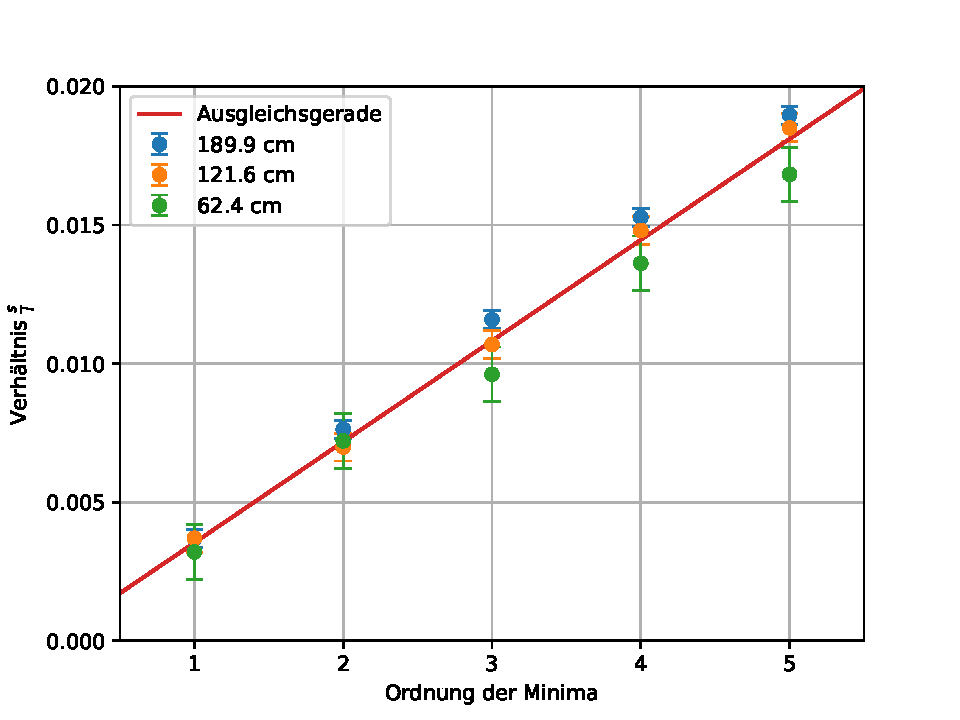
\includegraphics[width=0.8\textwidth]{./plots/einzelspalt.pdf}
        \caption{Messergebnisse des Einzelspalts}
        \label{fig:einzelspalt}
    \end{figure}

    \bibliographystyle{plain}
    \bibliography{literature}

\end{document}